\section{Het requirements model: use-case diagram}

Tijdens de requirements modellering fase, worden de gewenste functionaliteiten uitgetekend. Hierbij wordt beschreven wat die functionaliteiten zijn, wie ze mag uitvoeren en wat hun beschrijving is.

Modelleren met use-cases werd ontwikkeld door Ivar Jacobson (1994) en is gebaseerd op de OOSE en Objectory methoden. Het is een bekende techniek voor de inventarisatie van de eisen van een systeem vanuit het standpunt van de externe gebruiker (de actor). Met deze techniek kan aangegeven worden wat een bestaand systeem doet of wat een nieuw systeem zal moeten doen.

\subsection{Examenvraag}

Net als een klassendiagram wordt het in een \textbf{iteratief} proces opgebouwd waarbij voortdurend overleg met de business professionals noodzakelijk is. 

Bij het modelleren met use-cases is het belangrijk dat het systeem gezien wordt als een \textcolor{red}{zwarte doos (black box)} die use-cases levert. 

\textbf{\href{https://nl.wikipedia.org/wiki/Zwarte_doos}{link: Zwarte doos of black box wikipedia}}

\textbf{\href{https://nl.wikipedia.org/wiki/Use_case}{link: use case wikipedia}}

\href{https://en.wikipedia.org/wiki/Use_case#Design_scopes}{Wikipedia: engels: black box vs white box}



Hierbij is het niet belangrijk hoe de use-cases intern werken en hoe zij geïmplementeerd worden. Verder in dit hoofdstuk wordt beschreven welke stappen hierbij ondernomen worden.

Een use-case diagram toont een aantal externe actoren (iets of iemand die interageert met het systeem, hetzij door een bepaalde actie te vragen of doordat bepaalde uitvoer daaraan afgeleverd moet worden) en hun connectie met de use-cases van het systeem. 

Een use-case is een door het systeem geleverde functionaliteit (dit is een manier waarop het systeem gebruikt kan worden) en wordt beschreven vanuit het \textbf{zichtpunt} van die actor. 

In het use-case diagram worden deze verbanden getoond, maar de eigenlijke beschrijving van een use-case gebeurt tekstueel (in UML vormt deze tekst een documentatiekenmerk van het modelelement), of kan weergegeven worden in een sequentie- of collaboratiediagram.
\newpage
De belangrijkste \textbf{doelstellingen} van het use-case diagram zijn:

\begin{itemize}
    \item elke use-case beschrijft één functionaliteit van het systeem, en resulteert uit een overeenstemming tussen de klant en de ontwikkelaars
    \item elke use-case is opgesteld vanuit het zichtpunt van de actor en NIET vanuit het systeem. Elke use-case beschrijft dus WAT er gebeurt en NIET HOE dat zal gebeuren.
    \item Het use-case diagram moet een duidelijke, consistente beschrijving vormen van wat het systeem moet doen, zodat het gedurende de ganse systeemontwikkeling als richtlijn kan fungeren.
    \item Het use-case diagram vormt ook de basis bij het opstellen van de systeem- en acceptatietest, aangezien het een duidelijk beeld geeft van de systeemeisen.
    \item Een use-case wordt altijd geïnitieerd door een actor en levert altijd een waarde op voor een actor. Dit kan dezelfde actor zijn, maar kan ook een andere actor zijn.
    \item Een use-case moet altijd compleet zijn. Het is niet mogelijk om een use-case gedeeltelijk uit te voeren. 
    \item Een use-case wordt beschreven in één of meerdere scenario's. Elk scenario is een reeks van interacties tussen één of meerdere actoren en het systeem.
\end{itemize}

\subsection{Relaties tussen use-cases}

Er bestaan drie soorten relaties tussen use-cases. Dit zijn verschillende vormen van overerving :

\subsubsection{Extends relatie}

Dit is een generalisatie relatie waarin een use-case een andere use-case uitbreidt door aan een algemene use-case acties toe te voegen. 

De uitbreidende use-case kan gedrag omvatten van de use-case die uitgebreid wordt, afhankelijk van de voorwaarden van de uitbreiding. De use-case hoeft niet noodzakelijk het volledige gedrag van de andere te omvatten, de use-case kan zelf kiezen welk gedrag van de algemene use-case hergebruikt wordt.

\subsubsection{Uses-relatie}

Dit is een generalisatie relatie waarin een use-case een andere use-case gebruikt, waarbij aangegeven wordt dat het gedrag van de algemene use-case eveneens als deel van de gespecialiseerde use-case. Let op: als een use-case een andere use-case gebruikt, moet die volledig gebruikt worden. Als de gebruikte use-case nooit zelfstandig als use-case gebruikt wordt, wordt deze een abstracte use-case genoemd.

\subsubsection{Groepering}

Als een aantal use-cases gelijksoortige functionaliteiten afhandelen of op een andere manier verbonden zijn, kunnen ze in een package gebundeld worden (zie eerder).
Een package heeft op zich geen semantische betekenis, maar biedt een mogelijkheid om eisen in categorieën in te delen.
\newpage
\subsubsection{Generalisatie}
Tussen use-cases kunnen generalisatieverbanden bestaan. In deze situatie wordt in de superklasse aangegeven wat de algemene functionaliteit is. In de sub-case wordt beschreven wat er anders is in dit specifieke geval ten opzichten van de algemene functionaliteit.

%afbeelding nog plaatsen

\begin{center}
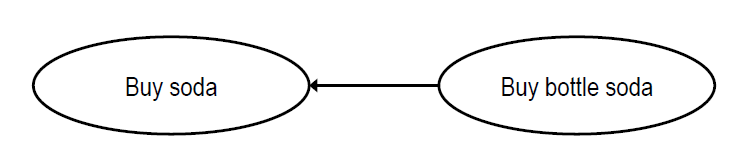
\includegraphics[width=4in]{img/generalisatie}%
\end{center}

Ook tussen actoren kunnen generalisatieverbanden bestaan. Deze situatie doet zich voor als verschillende actors ook een meer algemene rol spelen. Dit verband wordt voorgesteld door een lijn met lege driehoek aan de kant van de superklasse.

%afbeelding nog plaatsen

\begin{center}
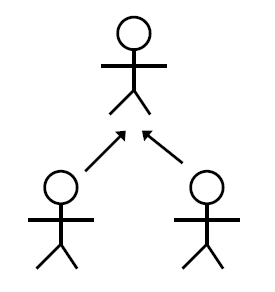
\includegraphics[width=2in]{img/genact}%
\end{center}

\subsection{Concepten van het use-case diagram}

Bij het opmaken van een use-case diagram, zijn de volgende concepten heel belangrijk:

\subsubsection{Het systeem}

Een belangrijk onderdeel bij het modelleren met behulp van use-cases is het afbakenen van het systeem: wat zijn de systeemgrenzen en wat zijn de functionaliteiten die het systeem moet kunnen vervullen.

%afbeelding nog plaatsen

\begin{comment}
\begin{center}
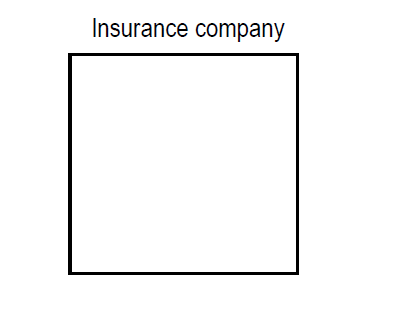
\includegraphics[width=2in]{img/scope}%
\end{center}
\end{comment}

\begin{wrapfigure}[10]{r}{0.5\textwidth}
  \begin{center}
    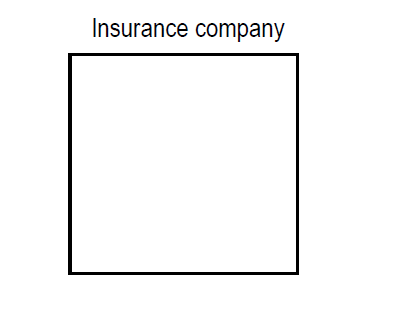
\includegraphics[width=0.28\textwidth]{img/scope}
  \end{center}
\end{wrapfigure}

In het use-case diagram wordt het systeem aangeduid door een vierkant: alles wat erbinnen ligt, behoort tot het systeem. Wat erbuiten ligt, behoort tot de systeemomgeving.

Let op: het afbakenen van het systeem is niet eenvoudig omdat het niet altijd duidelijk is welke functionaliteiten door het systeem uitgevoerd moeten worden of beter handmatig of door andere systemen kunnen gebeuren. Bovendien kunnen deze veranderen al naargelang de vorderingen bij de ontwikkeling van het systeem: in eerste instantie kan beperkt worden tot de basisfuncties en op het moment dat die redelijk stabiel zijn, kunnen de functionaliteiten verder uitgebreid worden.

\subsubsection{De actor : mogelijke examenvraag op examenwiki}

Een actor is iets of iemand die in interactie treedt met het systeem. Een actor is altijd een type, nooit een instantie. De actor zal berichten sturen naar het systeem of berichten van het systeem ontvangen, of met andere woorden informatie met het systeem uitwisselen. Een actor zal use-cases uitvoeren. Het kan een mens zijn, maar ook een ander systeem. Het representeert in ieder geval een rol en niet een individuele gebruiker van het systeem. Iemand kan een bepaalde rol vervullen voor de ene use-case en een andere rol voor een andere use-case. In die hoedanigheid is die persoon dus in feite meerdere actoren... Zo kan er ook een onderscheid gemaakt worden tussen actieve (die de use-case initiëren) en passieve (die nooit een use-case opstarten, maar er alleen maar aan deelnemen) actoren.
De actor communiceert met het systeem door het versturen en ontvangen van berichten.

De naam van de actor representeert de rol die de actor speelt voor die use- case.

%afbeelding nog plaatsen

\begin{center}
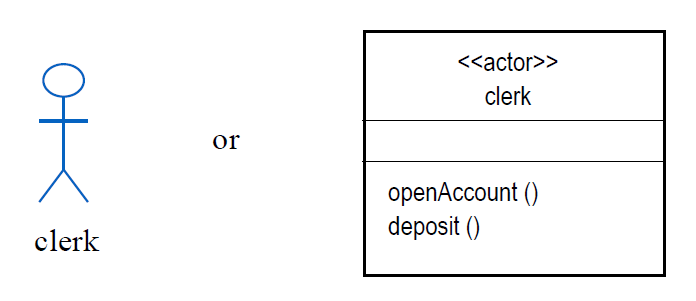
\includegraphics[width=4in]{img/actor3}%
\end{center}

Een actor wordt in het use-case diagram voorgesteld door een draadpoppetje of als klasse met stereotype actor (zie ook slide).
\newpage
\subsubsection{De use-case}

Een use-case stelt een volledige functionaliteit voor zoals die waargenomen wordt door een actor. Het wordt gedefinieerd als een verzameling sequenties die door het systeem uitgevoerd moeten worden en voor een actor een waarneembaar resultaat opleveren.

%afbeelding nog plaatsen

\begin{center}
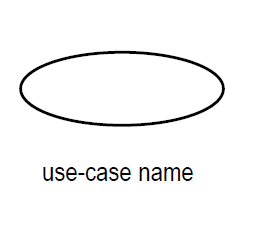
\includegraphics[width=4in]{img/usecase1}%
\end{center}

De use-case wordt in het diagram voorgesteld als een ellips met daarin de naam van de use-case, maar wordt in een tekstuele vorm beschreven als sequentie van acties die door het systeem ondernomen moeten worden en een waarneembaar resultaat opleveren voor de actor.

Een use-case wordt altijd geïnitieerd door een actor en moet een waarde opleveren voor een actor (dit kan desnoods een andere actor zijn). Een use-case moet bovendien compleet zijn. De use-case is pas volledig als de eindwaarde geproduceerd is.
Use-cases zijn verbonden met actoren via communicatie-associaties. Deze associaties laten zien welke actoren met welke use-cases communiceren.
\newpage
\subsection{Beschrijving van de use-case}

Een use-case kan beschreven worden in een activiteitendiagram (komt verder in deze tekst aan bod), maar deze beschrijving gebeurt meestal tekstueel.

%afbeelding nog plaatsen

\begin{center}
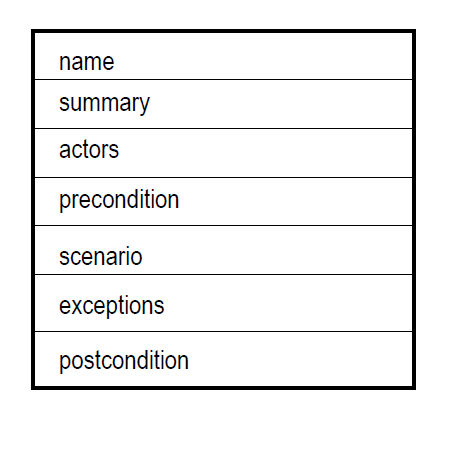
\includegraphics[width=4.5in]{img/usecase2}%
\end{center}

\begin{itemize}
    \item Naam
    
    Deze duidt op een unieke manier aan hoe de use-case aangeduid kan worden. Deze naam moet uiteraard de zelfde zijn als de naam aangeduid in het use- case diagram.
    \item Samenvatting
    
    Hier wordt beschreven wat de uiteindelijke doelstelling is van de use-case: een use-case is heel doelgericht en dit doel moet heel duidelijk zijn.
    \item Actoren
    
    Wie komt in contact met de use-case? Dit wil zeggen: welke actoren initiëren de use-case en / of komen ermee in contact.
    \item Aannamen
    
    Welke eisen moeten voldaan zijn vooraleer de use-case opgestart wordt? Deze worden ook dikwijls de \textbf{precondities} genoemd.
    
In deze aannamen wordt een soort contract opgesteld met de eindgebruiker: als deze condities niet voldaan zijn, mag de use-case zelf niet opgestart worden.
    \item Beschrijving
    
    Het scenario: welke berichten worden uitgewisseld met welke actoren en welke interactiestappen moeten hierbij ondernomen worden?
    
    Let wel op dat deze opsomming van deze interactiestappen gebeurt vanuit het \textbf{zichtpunt} van de actor en \textbf{niet} vanuit het systeem. Er wordt steeds uitgegaan van de normale gang van zaken.
    
    Wel wordt in de beschrijving aangegeven \textbf{wanneer} in welke omstandigheden van deze normale gang van zaken afgeweken wordt.
    
    Als aanvulling (maar niet als vervanging) op deze beschrijving kan ook gewerkt worden met scenario's om specifieke gevallen uit te breiden.
    \item Uitzonderingen
    
    Om het overzicht van de interactiestappen eenvoudiger te houden worden de uitzonderingstoestanden niet opgenomen maar afzonderlijk opgesomd.
    
    Daardoor kan in de beschrijving beperkt worden tot de normale gang van zaken. 
    
    In de uitzonderingen wordt beschreven wat de afwijking is ten opzichte van de normale gang van zaken en wat er moet gebeuren als deze uitzonderingstoestand zich voordoet.
    
    \item resultaat
    
    Hier wordt beschreven hoe de use-case eindigt met een bericht naar de actor. 
    
    Dit wordt ook de \textbf{postconditie} genoemd.
    
    In het contract met de eindgebruiker wordt hier beschreven wat de \textbf{eindsituatie is na uitvoering van de use-case.}
\end{itemize}
\newpage
\subsection{Werkwijze}

Het eigenlijke werk gaat over een definitie van het systeem, onderzoek naar de actoren en de use-cases, een beschrijving van die use-cases, de definitie van de relatie tussen de use-cases en een validatie van het model.

\begin{itemize}
\item \textbf{Identificeer de grens van het systeem en vind de actoren}

Om de actoren te definiëren, wordt een studie gemaakt van het huidige systeem waarbij gekeken wordt welke verschillende rollen de business professionals vervullen bij het uitvoeren van hun dagelijkse taken.

De actoren kunnen geïdentificeerd worden door een aantal vragen te beantwoorden: 
\begin{itemize}
    \item Wie gebruikt de hoofdfunctionaliteiten van het systeem? 
    \item Wie heeft het systeem nodig voor de ondersteuning van zijn dagelijkse activiteiten? 
    \item Wie moet het systeem onderhouden? 
    \item Met welke soft- en hardware moet het systeem werken?
    \item Wie is er geïnteresseerd in de resultaten die door ons systeem gegenereerd worden?
\end{itemize}

\item \textbf{Vind de use-cases voor iedere actor}

Het zoeken naar use-cases begint bij de eerder gevonden actoren. Voor elke actor moet de vraag gesteld worden welke functionaliteiten die actor nodig heeft van het systeem en wil hij gegevens lezen, wijzigen, verwijderen of opslaan?
Bepaal de aannamen voor elke use-case
\item \textbf{Bepaal de interactiestappen voor elke use-case}

Hier wordt een overzicht gegeven van alle stappen die doorlopen worden in de use-case.
\item \textbf{Bepaal de mogelijke uitzonderingen voor elke use-case}

Hier wordt een overzicht gegeven van welke uitzonderingen zich kunnen voordoen en hoe ze opgelost kunnen worden.
\item \textbf{Splits veel voorkomende subcases uit}

Ga na of in de beschreven use-cases een aantal subcases kunnen onderscheiden worden. Zo ja, beschrijf die dan op dezelfde manier.
\item \textbf{Maak het use-case diagram}

Maak een overzicht van de use-cases in een use-case diagram.
\item \textbf{Test de use-cases}

Een goede techniek om de use-cases te testen is het doorlopen (walk through) van de use-cases (walking the use-case). Hierbij spelen verschillende mensen de actoren en het systeem. De persoon die de initiërende actor speelt begint met zeggen wat het systeem moet doen. Daarna worden de beschreven interactiestappen doorlopen en wordt op die manier gecontroleerd of de beschrijving klopt.

\end{itemize}

